

% Gradient Info
  
\tikzset {_ectzm6pjz/.code = {\pgfsetadditionalshadetransform{ \pgftransformshift{\pgfpoint{9.5 bp } { 15.5 bp }  }  \pgftransformscale{1 }  }}}
\pgfdeclareradialshading{_ahugjddyw}{\pgfpoint{0bp}{0bp}}{rgb(0bp)=(1,1,1);
rgb(0bp)=(1,1,1);
rgb(25bp)=(0.82,0.01,0.11);
rgb(400bp)=(0.82,0.01,0.11)}

% Gradient Info
  
\tikzset {_th1cm3in6/.code = {\pgfsetadditionalshadetransform{ \pgftransformshift{\pgfpoint{9.5 bp } { 15.5 bp }  }  \pgftransformscale{1 }  }}}
\pgfdeclareradialshading{_d1dtwgk5f}{\pgfpoint{0bp}{0bp}}{rgb(0bp)=(1,1,1);
rgb(0bp)=(1,1,1);
rgb(25bp)=(0.97,0.91,0.11);
rgb(400bp)=(0.97,0.91,0.11)}

% Gradient Info
  
\tikzset {_zhr1fu2w4/.code = {\pgfsetadditionalshadetransform{ \pgftransformshift{\pgfpoint{9.5 bp } { 15.5 bp }  }  \pgftransformscale{1 }  }}}
\pgfdeclareradialshading{_1ut9eedgr}{\pgfpoint{0bp}{0bp}}{rgb(0bp)=(1,1,1);
rgb(0bp)=(1,1,1);
rgb(25bp)=(0.72,0.91,0.53);
rgb(400bp)=(0.72,0.91,0.53)}
\tikzset{_809g6ggoh/.code = {\pgfsetadditionalshadetransform{\pgftransformshift{\pgfpoint{9.5 bp } { 15.5 bp }  }  \pgftransformscale{1 } }}}
\pgfdeclareradialshading{_nd18wnqfs} { \pgfpoint{0bp} {0bp}} {color(0bp)=(transparent!0);
color(0bp)=(transparent!0);
color(25bp)=(transparent!50);
color(400bp)=(transparent!50)} 
\pgfdeclarefading{_5lgbtl41j}{\tikz \fill[shading=_nd18wnqfs,_809g6ggoh] (0,0) rectangle (50bp,50bp); } 

% Gradient Info
  
\tikzset {_0mv3s2zfu/.code = {\pgfsetadditionalshadetransform{ \pgftransformshift{\pgfpoint{9.5 bp } { 15.5 bp }  }  \pgftransformscale{1 }  }}}
\pgfdeclareradialshading{_byc674lfj}{\pgfpoint{0bp}{0bp}}{rgb(0bp)=(1,1,1);
rgb(0bp)=(1,1,1);
rgb(25bp)=(0.29,0.56,0.89);
rgb(400bp)=(0.29,0.56,0.89)}
\tikzset{_kgqqhn495/.code = {\pgfsetadditionalshadetransform{\pgftransformshift{\pgfpoint{9.5 bp } { 15.5 bp }  }  \pgftransformscale{1 } }}}
\pgfdeclareradialshading{_iqidbwe0j} { \pgfpoint{0bp} {0bp}} {color(0bp)=(transparent!0);
color(0bp)=(transparent!0);
color(25bp)=(transparent!50);
color(400bp)=(transparent!50)} 
\pgfdeclarefading{_zuztfk56c}{\tikz \fill[shading=_iqidbwe0j,_kgqqhn495] (0,0) rectangle (50bp,50bp); } 

% Gradient Info
  
\tikzset {_iddht9xy5/.code = {\pgfsetadditionalshadetransform{ \pgftransformshift{\pgfpoint{9.5 bp } { 15.5 bp }  }  \pgftransformscale{1 }  }}}
\pgfdeclareradialshading{_96md7qt0n}{\pgfpoint{0bp}{0bp}}{rgb(0bp)=(1,1,1);
rgb(0bp)=(1,1,1);
rgb(25bp)=(0.82,0.01,0.11);
rgb(400bp)=(0.82,0.01,0.11)}

% Gradient Info
  
\tikzset {_upwrgh5t1/.code = {\pgfsetadditionalshadetransform{ \pgftransformshift{\pgfpoint{9.5 bp } { 15.5 bp }  }  \pgftransformscale{1 }  }}}
\pgfdeclareradialshading{_1vnog2y7n}{\pgfpoint{0bp}{0bp}}{rgb(0bp)=(1,1,1);
rgb(0bp)=(1,1,1);
rgb(25bp)=(0.29,0.56,0.89);
rgb(400bp)=(0.29,0.56,0.89)}

% Gradient Info
  
\tikzset {_o60vc6flc/.code = {\pgfsetadditionalshadetransform{ \pgftransformshift{\pgfpoint{9.5 bp } { 15.5 bp }  }  \pgftransformscale{1 }  }}}
\pgfdeclareradialshading{_7owy0tp3f}{\pgfpoint{0bp}{0bp}}{rgb(0bp)=(1,1,1);
rgb(0bp)=(1,1,1);
rgb(25bp)=(0.97,0.91,0.11);
rgb(400bp)=(0.97,0.91,0.11)}

% Gradient Info
  
\tikzset {_u7bjhmdgn/.code = {\pgfsetadditionalshadetransform{ \pgftransformshift{\pgfpoint{9.5 bp } { 15.5 bp }  }  \pgftransformscale{1 }  }}}
\pgfdeclareradialshading{_fat2eyov2}{\pgfpoint{0bp}{0bp}}{rgb(0bp)=(1,1,1);
rgb(0bp)=(1,1,1);
rgb(25bp)=(0.72,0.91,0.53);
rgb(400bp)=(0.72,0.91,0.53)}
\tikzset{every picture/.style={line width=0.75pt}} %set default line width to 0.75pt        

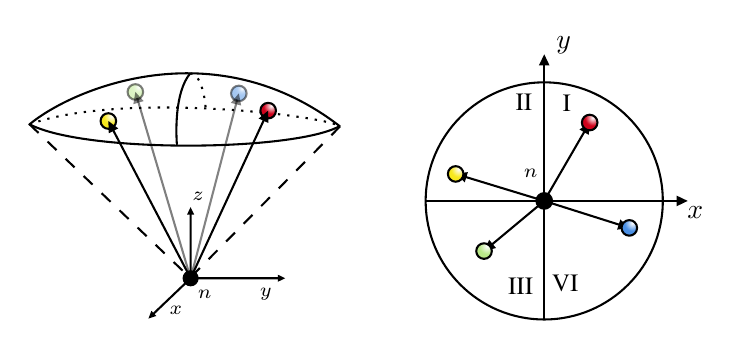
\begin{tikzpicture}[x=0.75pt,y=0.75pt,yscale=-1,xscale=1]
%uncomment if require: \path (0,300); %set diagram left start at 0, and has height of 300

%Straight Lines [id:da6622258070253217] 
\draw    (399.47,155.63) -- (437.62,167.72) ;
\draw [shift={(440.47,168.63)}, rotate = 197.59] [fill={rgb, 255:red, 0; green, 0; blue, 0 }  ][line width=0.08]  [draw opacity=0] (5.36,-2.57) -- (0,0) -- (5.36,2.57) -- cycle    ;
%Straight Lines [id:da2311108883972648] 
\draw    (399.47,155.63) -- (419.87,120.45) ;
\draw [shift={(421.37,117.86)}, rotate = 120.11] [fill={rgb, 255:red, 0; green, 0; blue, 0 }  ][line width=0.08]  [draw opacity=0] (5.36,-2.57) -- (0,0) -- (5.36,2.57) -- cycle    ;
%Straight Lines [id:da8545661798579438] 
\draw    (399.47,155.63) -- (359.68,143.5) ;
\draw [shift={(356.81,142.63)}, rotate = 16.95] [fill={rgb, 255:red, 0; green, 0; blue, 0 }  ][line width=0.08]  [draw opacity=0] (5.36,-2.57) -- (0,0) -- (5.36,2.57) -- cycle    ;
%Straight Lines [id:da09133942459342603] 
\draw    (399.47,155.63) -- (372.78,177.87) ;
\draw [shift={(370.47,179.79)}, rotate = 320.19] [fill={rgb, 255:red, 0; green, 0; blue, 0 }  ][line width=0.08]  [draw opacity=0] (5.36,-2.57) -- (0,0) -- (5.36,2.57) -- cycle    ;
%Curve Lines [id:da3408986332399885] 
\draw    (151.5,118.74) .. controls (171.93,101.66) and (240.27,72.66) .. (301.1,119.74) ;
%Shape: Boxed Bezier Curve [id:dp96148792342119] 
\draw    (151.1,118.49) .. controls (164.79,125.97) and (199.55,129.31) .. (232.6,128.97) .. controls (244.14,128.85) and (255.47,128.28) .. (265.62,127.29) .. controls (281.63,125.73) and (294.73,123.1) .. (301.1,119.49) ;
%Shape: Circle [id:dp6133467460873314] 
\draw  [fill={rgb, 255:red, 0; green, 0; blue, 0 }  ,fill opacity=1 ] (225.73,192.89) .. controls (225.73,191.03) and (227.24,189.52) .. (229.11,189.52) .. controls (230.97,189.52) and (232.48,191.03) .. (232.48,192.89) .. controls (232.48,194.76) and (230.97,196.27) .. (229.11,196.27) .. controls (227.24,196.27) and (225.73,194.76) .. (225.73,192.89) -- cycle ;
%Straight Lines [id:da43451900166447055] 
\draw  [dash pattern={on 4.5pt off 4.5pt}]  (151.5,118.74) -- (229.11,192.89) ;
%Straight Lines [id:da27796655259699965] 
\draw  [dash pattern={on 4.5pt off 4.5pt}]  (301.1,119.74) -- (226.97,194.62) ;
%Straight Lines [id:da6999128942682394] 
\draw    (229.11,192.89) -- (271.68,192.88) ;
\draw [shift={(274.68,192.88)}, rotate = 179.98] [fill={rgb, 255:red, 0; green, 0; blue, 0 }  ][line width=0.08]  [draw opacity=0] (3.57,-1.72) -- (0,0) -- (3.57,1.72) -- cycle    ;
%Straight Lines [id:da9362945852514719] 
\draw    (229.09,161.63) -- (229.11,192.89) ;
\draw [shift={(229.09,158.63)}, rotate = 89.97] [fill={rgb, 255:red, 0; green, 0; blue, 0 }  ][line width=0.08]  [draw opacity=0] (3.57,-1.72) -- (0,0) -- (3.57,1.72) -- cycle    ;
%Straight Lines [id:da19983983435889585] 
\draw    (210.97,210.22) -- (229.11,192.89) ;
\draw [shift={(208.8,212.29)}, rotate = 316.31] [fill={rgb, 255:red, 0; green, 0; blue, 0 }  ][line width=0.08]  [draw opacity=0] (3.57,-1.72) -- (0,0) -- (3.57,1.72) -- cycle    ;
%Curve Lines [id:da5161113958018073] 
\draw  [dash pattern={on 0.84pt off 2.51pt}]  (151.5,118.74) .. controls (195.95,102.58) and (294.93,114.66) .. (301.1,119.74) ;
%Shape: Circle [id:dp34975665552264834] 
\path  [shading=_ahugjddyw,_ectzm6pjz] (262.72,112.13) .. controls (262.72,110.05) and (264.4,108.38) .. (266.47,108.38) .. controls (268.55,108.38) and (270.22,110.05) .. (270.22,112.13) .. controls (270.22,114.2) and (268.55,115.88) .. (266.47,115.88) .. controls (264.4,115.88) and (262.72,114.2) .. (262.72,112.13) -- cycle ; % for fading 
 \draw   (262.72,112.13) .. controls (262.72,110.05) and (264.4,108.38) .. (266.47,108.38) .. controls (268.55,108.38) and (270.22,110.05) .. (270.22,112.13) .. controls (270.22,114.2) and (268.55,115.88) .. (266.47,115.88) .. controls (264.4,115.88) and (262.72,114.2) .. (262.72,112.13) -- cycle ; % for border 

%Straight Lines [id:da015689949749956855] 
\draw    (229.11,192.89) -- (265.22,114.85) ;
\draw [shift={(266.47,112.13)}, rotate = 114.83] [fill={rgb, 255:red, 0; green, 0; blue, 0 }  ][line width=0.08]  [draw opacity=0] (5.36,-2.57) -- (0,0) -- (5.36,2.57) -- cycle    ;
%Shape: Circle [id:dp14790978690615875] 
\draw   (342.35,155.63) .. controls (342.35,124.08) and (367.93,98.5) .. (399.47,98.5) .. controls (431.02,98.5) and (456.6,124.08) .. (456.6,155.63) .. controls (456.6,187.17) and (431.02,212.75) .. (399.47,212.75) .. controls (367.93,212.75) and (342.35,187.17) .. (342.35,155.63) -- cycle ;
%Straight Lines [id:da6300963682328697] 
\draw    (399.47,88) -- (399.47,212.75) ;
\draw [shift={(399.47,85)}, rotate = 90] [fill={rgb, 255:red, 0; green, 0; blue, 0 }  ][line width=0.08]  [draw opacity=0] (5.36,-2.57) -- (0,0) -- (5.36,2.57) -- cycle    ;
%Straight Lines [id:da26734379961293575] 
\draw    (342.35,155.63) -- (465.6,155.63) ;
\draw [shift={(468.6,155.63)}, rotate = 180] [fill={rgb, 255:red, 0; green, 0; blue, 0 }  ][line width=0.08]  [draw opacity=0] (5.36,-2.57) -- (0,0) -- (5.36,2.57) -- cycle    ;
%Shape: Circle [id:dp2045150857945045] 
\draw  [fill={rgb, 255:red, 0; green, 0; blue, 0 }  ,fill opacity=1 ] (395.72,155.63) .. controls (395.72,153.55) and (397.4,151.88) .. (399.47,151.88) .. controls (401.55,151.88) and (403.22,153.55) .. (403.22,155.63) .. controls (403.22,157.7) and (401.55,159.38) .. (399.47,159.38) .. controls (397.4,159.38) and (395.72,157.7) .. (395.72,155.63) -- cycle ;
%Shape: Circle [id:dp6985238736959959] 
\path  [shading=_d1dtwgk5f,_th1cm3in6] (185.72,117.13) .. controls (185.72,115.05) and (187.4,113.38) .. (189.47,113.38) .. controls (191.55,113.38) and (193.22,115.05) .. (193.22,117.13) .. controls (193.22,119.2) and (191.55,120.88) .. (189.47,120.88) .. controls (187.4,120.88) and (185.72,119.2) .. (185.72,117.13) -- cycle ; % for fading 
 \draw   (185.72,117.13) .. controls (185.72,115.05) and (187.4,113.38) .. (189.47,113.38) .. controls (191.55,113.38) and (193.22,115.05) .. (193.22,117.13) .. controls (193.22,119.2) and (191.55,120.88) .. (189.47,120.88) .. controls (187.4,120.88) and (185.72,119.2) .. (185.72,117.13) -- cycle ; % for border 

%Shape: Circle [id:dp006151283675143171] 
\path  [shading=_1ut9eedgr,_zhr1fu2w4,path fading= _5lgbtl41j ,fading transform={xshift=2}] (198.72,103.13) .. controls (198.72,101.05) and (200.4,99.38) .. (202.47,99.38) .. controls (204.55,99.38) and (206.22,101.05) .. (206.22,103.13) .. controls (206.22,105.2) and (204.55,106.88) .. (202.47,106.88) .. controls (200.4,106.88) and (198.72,105.2) .. (198.72,103.13) -- cycle ; % for fading 
 \draw  [color={rgb, 255:red, 0; green, 0; blue, 0 }  ,draw opacity=0.5 ] (198.72,103.13) .. controls (198.72,101.05) and (200.4,99.38) .. (202.47,99.38) .. controls (204.55,99.38) and (206.22,101.05) .. (206.22,103.13) .. controls (206.22,105.2) and (204.55,106.88) .. (202.47,106.88) .. controls (200.4,106.88) and (198.72,105.2) .. (198.72,103.13) -- cycle ; % for border 

%Shape: Circle [id:dp7002763417470397] 
\path  [shading=_byc674lfj,_0mv3s2zfu,path fading= _zuztfk56c ,fading transform={xshift=2}] (248.58,103.84) .. controls (248.58,101.77) and (250.26,100.09) .. (252.33,100.09) .. controls (254.4,100.09) and (256.08,101.77) .. (256.08,103.84) .. controls (256.08,105.91) and (254.4,107.59) .. (252.33,107.59) .. controls (250.26,107.59) and (248.58,105.91) .. (248.58,103.84) -- cycle ; % for fading 
 \draw  [color={rgb, 255:red, 0; green, 0; blue, 0 }  ,draw opacity=0.5 ] (248.58,103.84) .. controls (248.58,101.77) and (250.26,100.09) .. (252.33,100.09) .. controls (254.4,100.09) and (256.08,101.77) .. (256.08,103.84) .. controls (256.08,105.91) and (254.4,107.59) .. (252.33,107.59) .. controls (250.26,107.59) and (248.58,105.91) .. (248.58,103.84) -- cycle ; % for border 

%Straight Lines [id:da7202474258526059] 
\draw    (229.11,192.89) -- (190.87,119.78) ;
\draw [shift={(189.47,117.13)}, rotate = 62.39] [fill={rgb, 255:red, 0; green, 0; blue, 0 }  ][line width=0.08]  [draw opacity=0] (5.36,-2.57) -- (0,0) -- (5.36,2.57) -- cycle    ;
%Straight Lines [id:da7608597927326616] 
\draw [color={rgb, 255:red, 0; green, 0; blue, 0 }  ,draw opacity=0.5 ]   (229.11,192.89) -- (203.33,106) ;
\draw [shift={(202.47,103.13)}, rotate = 73.48] [fill={rgb, 255:red, 0; green, 0; blue, 0 }  ,fill opacity=0.5 ][line width=0.08]  [draw opacity=0] (5.36,-2.57) -- (0,0) -- (5.36,2.57) -- cycle    ;
%Straight Lines [id:da3967042498113518] 
\draw [color={rgb, 255:red, 0; green, 0; blue, 0 }  ,draw opacity=0.49 ]   (229.11,192.89) -- (251.58,106.74) ;
\draw [shift={(252.33,103.84)}, rotate = 104.62] [fill={rgb, 255:red, 0; green, 0; blue, 0 }  ,fill opacity=0.49 ][line width=0.08]  [draw opacity=0] (5.36,-2.57) -- (0,0) -- (5.36,2.57) -- cycle    ;
%Shape: Circle [id:dp5842522612705374] 
\path  [shading=_96md7qt0n,_iddht9xy5] (417.62,117.86) .. controls (417.62,115.79) and (419.3,114.11) .. (421.37,114.11) .. controls (423.45,114.11) and (425.12,115.79) .. (425.12,117.86) .. controls (425.12,119.93) and (423.45,121.61) .. (421.37,121.61) .. controls (419.3,121.61) and (417.62,119.93) .. (417.62,117.86) -- cycle ; % for fading 
 \draw   (417.62,117.86) .. controls (417.62,115.79) and (419.3,114.11) .. (421.37,114.11) .. controls (423.45,114.11) and (425.12,115.79) .. (425.12,117.86) .. controls (425.12,119.93) and (423.45,121.61) .. (421.37,121.61) .. controls (419.3,121.61) and (417.62,119.93) .. (417.62,117.86) -- cycle ; % for border 

%Shape: Circle [id:dp40398487751084444] 
\path  [shading=_1vnog2y7n,_upwrgh5t1] (436.72,168.63) .. controls (436.72,166.55) and (438.4,164.88) .. (440.47,164.88) .. controls (442.55,164.88) and (444.22,166.55) .. (444.22,168.63) .. controls (444.22,170.7) and (442.55,172.38) .. (440.47,172.38) .. controls (438.4,172.38) and (436.72,170.7) .. (436.72,168.63) -- cycle ; % for fading 
 \draw  [color={rgb, 255:red, 0; green, 0; blue, 0 }  ,draw opacity=1 ] (436.72,168.63) .. controls (436.72,166.55) and (438.4,164.88) .. (440.47,164.88) .. controls (442.55,164.88) and (444.22,166.55) .. (444.22,168.63) .. controls (444.22,170.7) and (442.55,172.38) .. (440.47,172.38) .. controls (438.4,172.38) and (436.72,170.7) .. (436.72,168.63) -- cycle ; % for border 

%Shape: Circle [id:dp018365373284586428] 
\path  [shading=_7owy0tp3f,_o60vc6flc] (353.06,142.63) .. controls (353.06,140.55) and (354.74,138.88) .. (356.81,138.88) .. controls (358.88,138.88) and (360.56,140.55) .. (360.56,142.63) .. controls (360.56,144.7) and (358.88,146.38) .. (356.81,146.38) .. controls (354.74,146.38) and (353.06,144.7) .. (353.06,142.63) -- cycle ; % for fading 
 \draw   (353.06,142.63) .. controls (353.06,140.55) and (354.74,138.88) .. (356.81,138.88) .. controls (358.88,138.88) and (360.56,140.55) .. (360.56,142.63) .. controls (360.56,144.7) and (358.88,146.38) .. (356.81,146.38) .. controls (354.74,146.38) and (353.06,144.7) .. (353.06,142.63) -- cycle ; % for border 

%Shape: Circle [id:dp6099953585536941] 
\path  [shading=_fat2eyov2,_u7bjhmdgn] (366.72,179.79) .. controls (366.72,177.72) and (368.4,176.04) .. (370.47,176.04) .. controls (372.55,176.04) and (374.22,177.72) .. (374.22,179.79) .. controls (374.22,181.86) and (372.55,183.54) .. (370.47,183.54) .. controls (368.4,183.54) and (366.72,181.86) .. (366.72,179.79) -- cycle ; % for fading 
 \draw  [color={rgb, 255:red, 0; green, 0; blue, 0 }  ,draw opacity=1 ] (366.72,179.79) .. controls (366.72,177.72) and (368.4,176.04) .. (370.47,176.04) .. controls (372.55,176.04) and (374.22,177.72) .. (374.22,179.79) .. controls (374.22,181.86) and (372.55,183.54) .. (370.47,183.54) .. controls (368.4,183.54) and (366.72,181.86) .. (366.72,179.79) -- cycle ; % for border 

%Curve Lines [id:da09503531180183733] 
\draw    (222.5,128.58) .. controls (222.11,123.44) and (221.22,103.22) .. (229,94.08) ;
%Curve Lines [id:da7933859191697868] 
\draw  [dash pattern={on 0.84pt off 2.51pt}]  (229,94.08) .. controls (234.78,94.56) and (236.33,109) .. (236.33,111) ;

% Text Node
\draw (231.11,197) node [anchor=north west][inner sep=0.75pt]  [font=\scriptsize] [align=left] {$\displaystyle n$};
% Text Node
\draw (217.54,205) node [anchor=north west][inner sep=0.75pt]  [font=\scriptsize] [align=left] {$\displaystyle x$};
% Text Node
\draw (260.97,196) node [anchor=north west][inner sep=0.75pt]  [font=\scriptsize] [align=left] {$\displaystyle y$};
% Text Node
\draw (228.49,150) node [anchor=north west][inner sep=0.75pt]  [font=\scriptsize] [align=left] {$\displaystyle z$};
% Text Node
\draw (403.8,75) node [anchor=north west][inner sep=0.75pt]   [align=left] {$\displaystyle y$};
% Text Node
\draw (467,157) node [anchor=north west][inner sep=0.75pt]   [align=left] {$\displaystyle x$};
% Text Node
\draw (388.11,139) node [anchor=north west][inner sep=0.75pt]  [font=\scriptsize] [align=left] {$\displaystyle n$};
% Text Node
\draw (406.8,102.8) node [anchor=north west][inner sep=0.75pt]  [font=\small] [align=left] {{\fontfamily{ptm}\selectfont I}};
% Text Node
\draw (384.2,102.6) node [anchor=north west][inner sep=0.75pt]  [font=\small] [align=left] {{\fontfamily{ptm}\selectfont II}};
% Text Node
\draw (380.6,191) node [anchor=north west][inner sep=0.75pt]  [font=\small] [align=left] {{\fontfamily{ptm}\selectfont III}};
% Text Node
\draw (401.8,189.8) node [anchor=north west][inner sep=0.75pt]  [font=\small] [align=left] {{\fontfamily{ptm}\selectfont VI}};


\end{tikzpicture}
